
%*******************************************************************************
%*********************************** Second Chapter ***************************
%*******************************************************************************
%!TEX root = 0.main.tex

\section{Other samplings and other Discrete Laplacians}

[What we want from the Laplacian matrix]\\
In a Graph Spherical CNN we use the fact that when the sampling of the sphere is regular enough, the graph $W_{i j} = \exp {-\frac{\norm{x_i-x_j}^2}{4t}}$ is such that the corresponding graph Laplacian $\mathbf L_n^t=D-W$ has a spectrum that is close enough to the spectrum of $\triangle$ so that we can approximate a spherical convolution of a signal with a kernel with a multiplication of a polynomial of the discrete Laplacian $\sum_k \theta_k (\mathbf L_n^t)^k$ times the vector of the sampled signal $\mathbf f_i = f(x_i)$. 

[Stating the problem we want to solve]\\
In Chapter 2 we showed a way to construct $\mathbf L_n^t$ that well approximates $\triangle$ in the case of a much regular sampling of the sphere, HEALPix. In this Chapter we focus to others samplings less uniform than HEALPix. The sampling that we will use for our study, very used in applications, is the so called equiangular sampling. We observe that in this case the Heat Kernel Graph Laplacian matrix is not able to correctly approximate the continuous Laplace-Beltrami operator, due to the fact that the equiangular sampling samples some specific areas of the sphere more than others. Figure \ref{fig:equiangular distortion} well illustrates this bad behavior of the Heat Kernel Graph Laplacian. The sphere has been sampled irregularly, with many more samples near the poles than near the equator. The sampling is made by the vertices of the mesh. On the left we plot one spherical harmonic $Y_\ell^i$ of degree $\ell=4$ and on the right we plot the corresponding eigenvector of the HKGL. We can see that by sampling the poles more than the equator the eigenvectors end up being deformed and artificially compressed along the equator. The goal of this chapter is to find a way of building a discrete approximation $\mathbf L$ of the Laplace-Beltrami operator more robust to non uniform sampling than the Heat Kernel Graph Laplacian matrix $\mathbf L_n^t$ used so far.

\begin{wrapfigure}{r}{0.5\textwidth}
	\label{fig:equiangular distortion}
	\begin{center}
			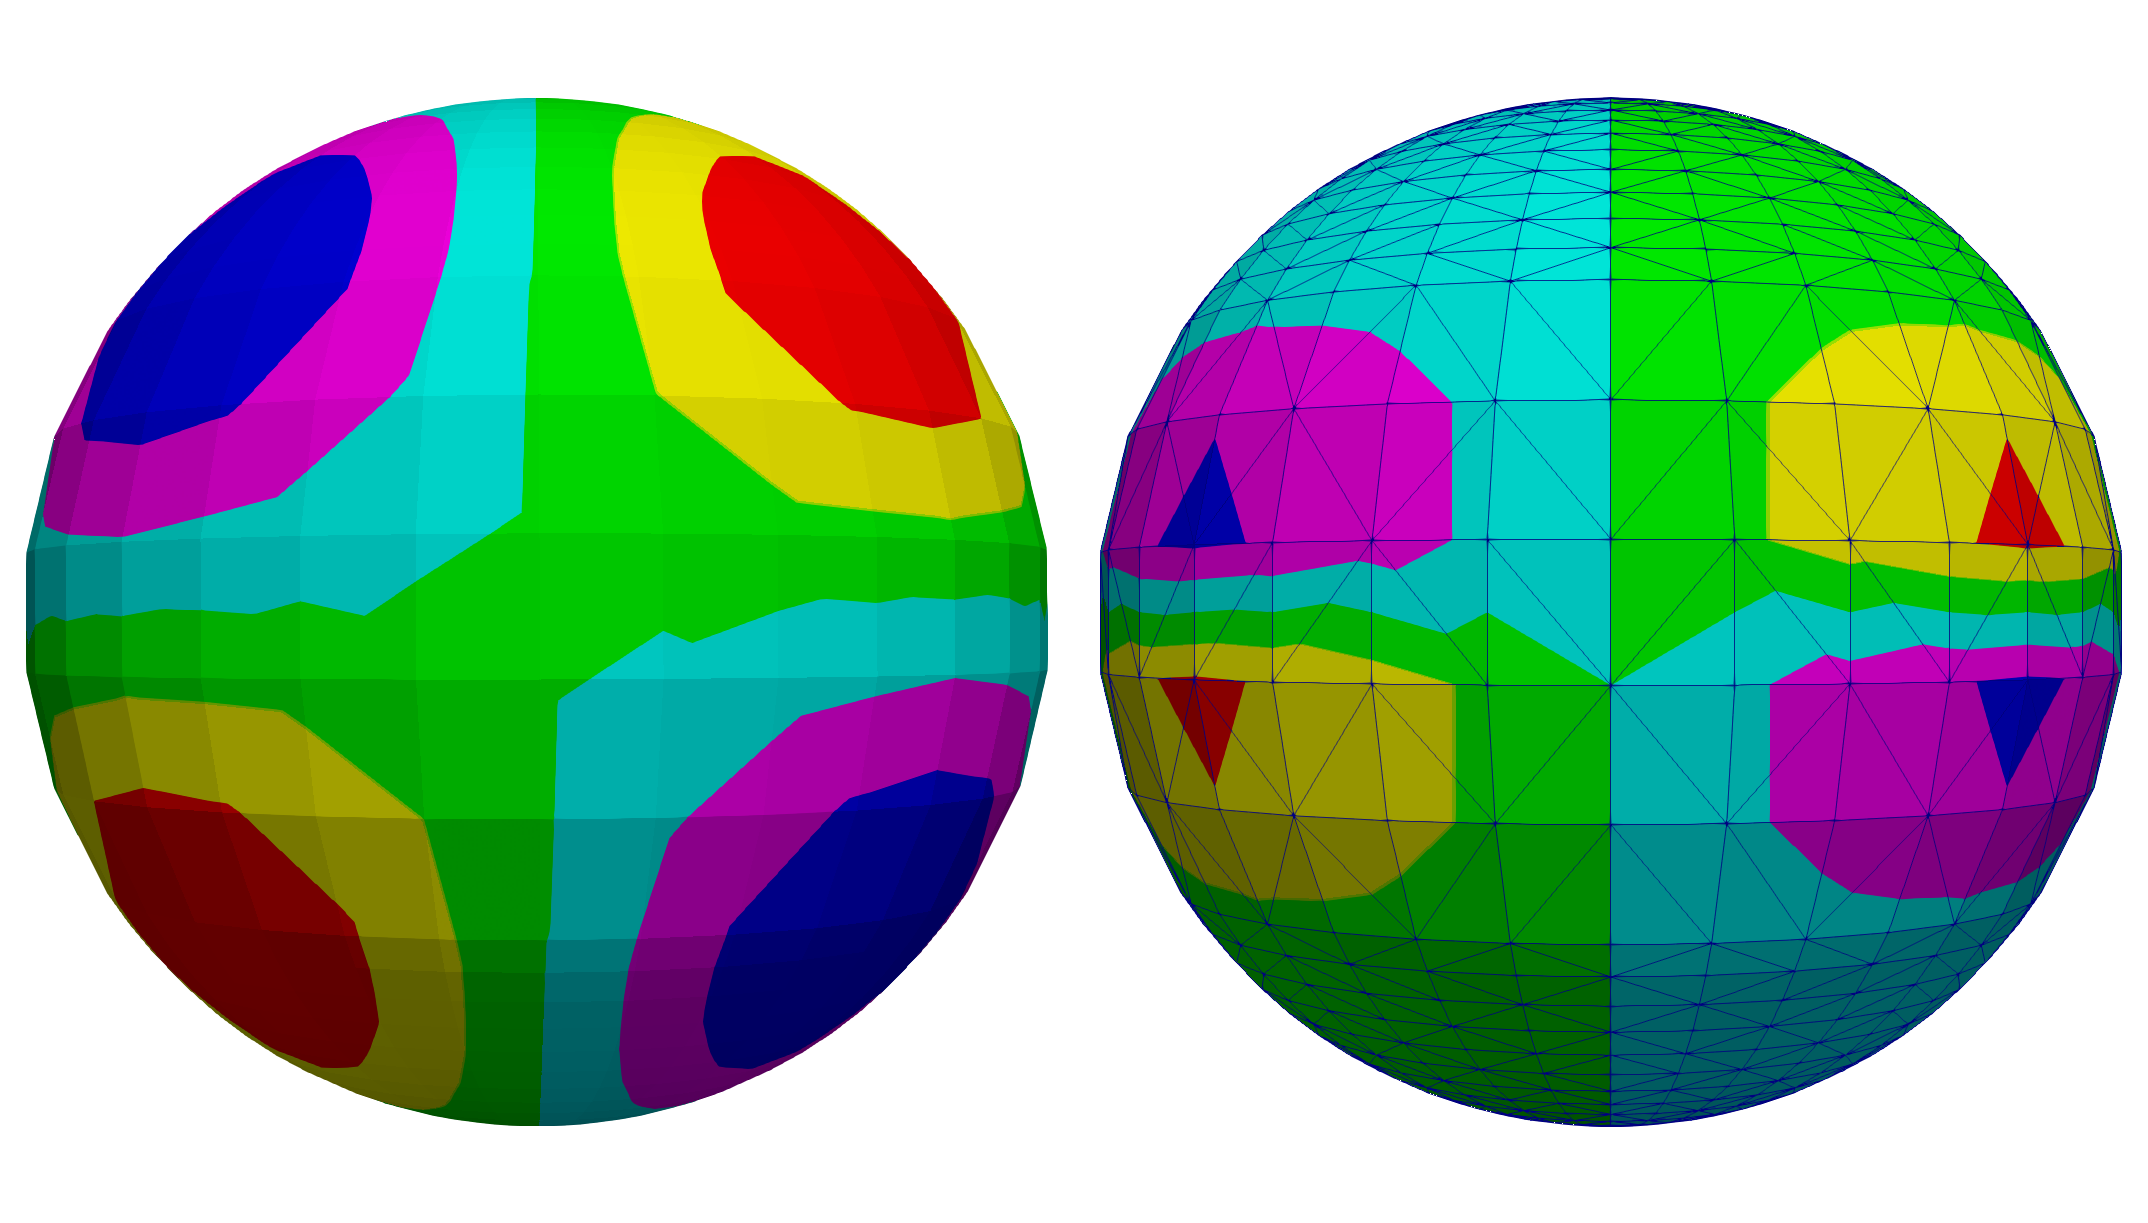
\includegraphics[width=0.5\textwidth]{../codes/04.imbalanced/img/confront_mixed.png}
	\end{center}
	\caption{On the left, the correct eigenmode. On the right: distortion of the eigenmode of the HKGL caused by an irregular sampling of the sphere.}
\end{wrapfigure}

[Say what we did to solve it]\\
This chapter is organized as follows: In Section \ref{sec:Chapter3: Heat Kernel Graph Laplacian on the Equiangular Sampling} we introduce the equiangular sampling and the results that we obtained with the Heat Kernel Graph Laplacian matrix. In Section \ref{sec:Chapter3: other discrete laplacians} we present a short overview of different ways of building an discrete approximation of the Laplace-Beltrami operator; in Section \ref{sec:Chapter3: Using the Finite Element Method to approximate the Laplace-Beltrami operator on a manifold} we deepen how to use the Finite Element Method (FEM) to construct a discrete approximation of $\triangle$ and how this way of constructing $\mathbf L$  is actually capable of taking into account the non uniformity of the sampling and correct it. in Section \ref{sec:Chapter3: Results} we present and discuss the results obtained.
\subsection{Heat Kernel Graph Laplacian on the Equiangular Sampling}
\label{sec:Chapter3: Heat Kernel Graph Laplacian on the Equiangular Sampling}

\subsubsection{The Equiangular Sampling}

Given the usual parametrization $x = x(\theta, \phi)$ of the sphere
$$
\mathbb{S}^{2}=\left\{x=\left(x_{1}, x_{2}, x_{3}\right) \in \mathbb{R}^{3} :\|x\|_{\mathbb{R}^{3}}=\left(x_{1}^{2}+x_{2}^{2}+x_{3}^{2}\right)^{1 / 2}=1\right\}
$$

$$
x_{1}=\cos (\phi) \sin (\theta), \quad x_{2}=\sin (\phi) \sin (\theta), \quad x_{3}=\cos (\theta)
$$
Let $m\in\mathbb N$, the uniform sampling of bandwidth $b=2^m$ is given by 
$
x_{j k}^{(b)}=x\left(\theta_{j}^{(b)}, \phi_{k}^{(b)}\right)
$
where
$$
\theta_{j}^{(b)} :=\pi \frac{j}{2 b}, \quad \phi_{k}^{(b)} :=2 \pi \frac{k}{2 b}
$$
\begin{figure}[h!]
	\centering
	\label{fig:equiangular sampling}
	\caption{Equiangular sampling with bandwidth $n=16$}
	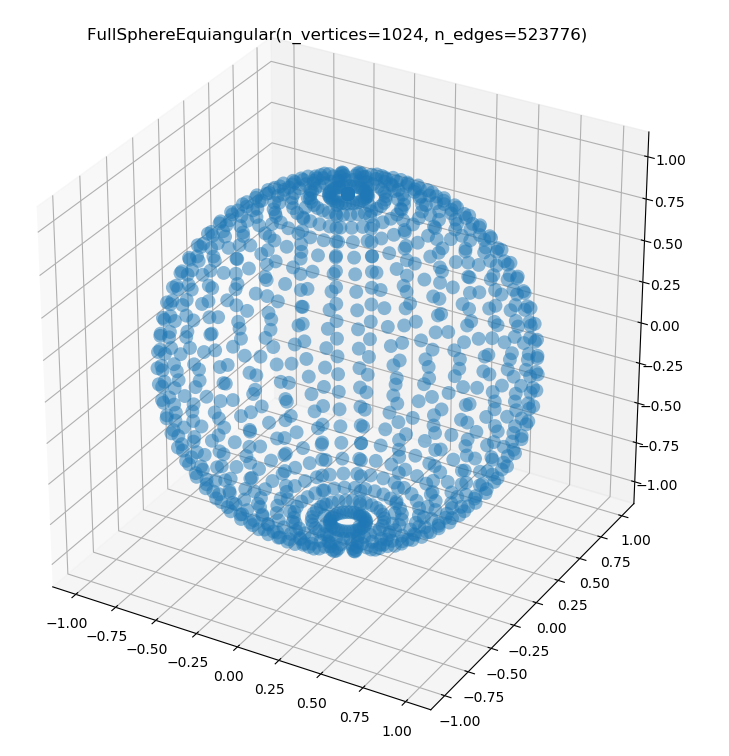
\includegraphics[width=0.5\textwidth]{../codes/02.HeatKernelGraphLaplacian/equiangular/equiangular.png}
\end{figure}
One has $n=4b^2$ points on the sphere, where $x_{0 k}^{(b)}$ corresponds to the north pole for every $k$. Notice also that the south pole is never sampled. In figure \ref{fig:equiangular sampling} it can also be appreciated how the area close to the poles is much more sampled that the equator. One reason for which this sampling is very useful is the following result from \cite{Driscoll:1994:CFT:184069.184073}, that states that any band limited function can be exactly recovered from its sampled values $f\left(x_{j k}^{(b)}\right)$:
\vspace{0.5cm}
\begin{prop}\label{prop:equiangular sampling theorem}
	Let \(l_{0} \in \mathbb{N}\) and \(m_{0} \in \mathbb{Z},\left|m_{0}\right| \leq l_{0} .\) If \(f=\sum_{l=0}^{b-1} \sum_{m=-l}^{l} \widehat{f}(l, m) Y_{l}^{m}\)
	then
	
	$$
	\begin{aligned} \widehat{f}\left(l_{0}, m_{0}\right)=& \frac{1}{4 b^{2}} \sum_{j=0}^{2 b-1} \sum_{k=0}^{2 b-1} f\left(x_{j k}^{(b)}\right) \overline{Y_{l_{0}}^{m_{0}}\left(x_{j k}^{(b)}\right)} \sin \left(\theta_{j}^{(b)}\right) \times \\ & \times \frac{4}{\pi} \sum_{l=0}^{b-1} \frac{1}{2 l+1} \sin \left((2 l+1) \theta_{j}^{(b)}\right) \end{aligned}
	$$
\end{prop}
\vspace{0.5cm}

\subsubsection{Heat Kernel Graph Laplacian}
Thanks to Proposition \ref{prop:equiangular sampling theorem}, assuming we can compute the Fourier transform of the eigenvectors of the Heat Kernel Graph Laplacian matrix and see how much they are aligned with the eigenspaces of the true Laplace-Beltrami operator. Here the results:


\begin{table}[h!]
	\centering
	\label{table:equiangular kernel width}
	\caption{Kernel width $t$ used to construct the Heat Kernel Graph Laplacian matrix fr each bandwidth $b$}
	\begin{tabular}{ c|c } 
	
$b$ & $t$ \\ 
	\hline
4 & 0.5 \\ 
8 & 0.3 \\ 
16 & 0.1 \\ 
	
	\end{tabular}
\end{table}

\begin{figure}[h!]
	\centering
	\label{fig:equiangular sampling alignment}
	\caption{Alignment of eigenspaces of the Heat Kernel Graph Laplacian matrix with the true Laplace-Beltrami eigenspaces on the equiangular sampling with $b=16$ and kernel width $t=0.1$}
	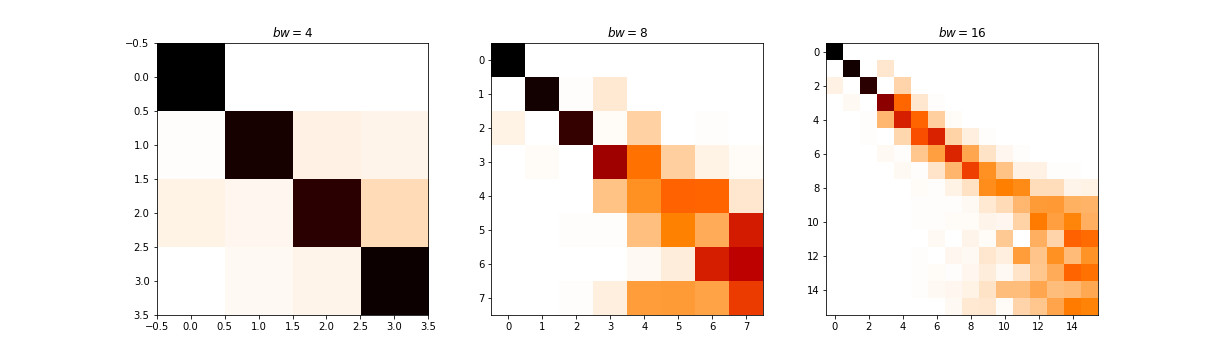
\includegraphics[width=0.9\textwidth]{../codes/02.HeatKernelGraphLaplacian/equiangular/equi_full.png}
\end{figure}
\begin{figure}[h!]
	\centering
	\label{fig:equiangular sampling alignment diagonal}
	\caption{Alignment of eigenspaces of the Heat Kernel Graph Laplacian matrix with the true Laplace-Beltrami eigenspaces on the equiangular sampling}
	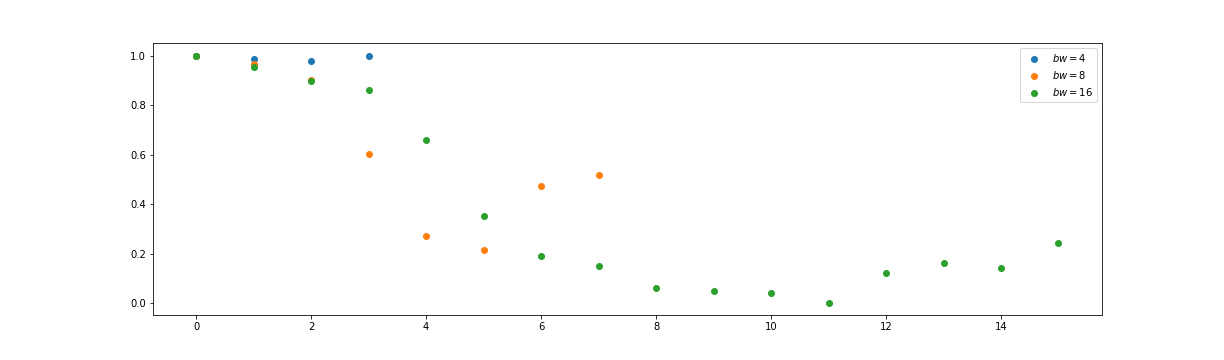
\includegraphics[width=0.9\textwidth]{../codes/02.HeatKernelGraphLaplacian/equiangular/equi_full_diagonal.png}
\end{figure}
\begin{figure}[h!]
	\centering
	\label{fig:equiangular sampling alignment eigenvalues}
	\caption{Eigenvalues of the Heat Kernel Graph Laplacian matrix on the equiangular sampling with $b=16$ and kernel width $t=0.1$}
	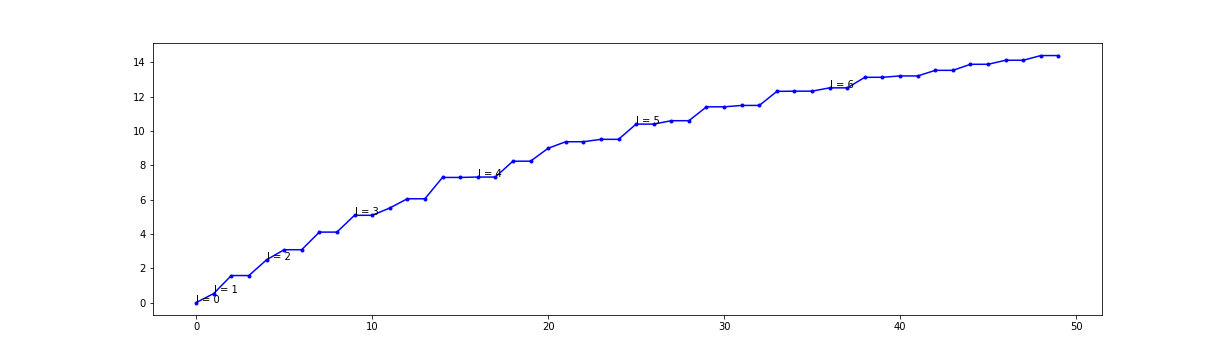
\includegraphics[width=0.9\textwidth]{../codes/02.HeatKernelGraphLaplacian/equiangular/equi_full_eigenvalues_16.png}
\end{figure}

It can be appreciated how poor these results are compared to the ones obtained with the HEALPix sampling. \\

[ Explain why they are so bad: Perspective of the quadrature formula]\\
A way to understand what's going on is the following: remembering the proof of theorem \ref{theo:pointwise convergence in the healpix case} and using again the notation $\phi^{t}(x ; y)=e^{-\frac{||x-y||^2}{4t}}\left(f(y)-f(x)\right)$, the key thing is to make $L_n^tf(y)=\sum_i \frac{1}{n} \phi^{t}(x_i ; y)$  approximate $L^tf(y)=\int_\mathcal M\phi^{t}(x ; y)d\mu(x)$, in other words we can see the graph weights as \textit{quadrature weights} meant to approximate the continuous integral on the right hand side of equation \ref{eq:quadrature approximation}.
\begin{equation}
\label{eq:quadrature approximation}
	\sum_i \frac{1}{n} \phi^{t}(x_i ; y) \quad \approxeq\quad \int_\mathcal M\phi^{t}(x ; y)d\mu(x)
\end{equation}
The way of building the graph of Belkin et al. works in the case of random sampling because in that way the sampling in the limit of the SLLN will sample the manifold uniformly, and thus there's no need of re-weighting the graph; in case of non uniform sampling, we intuitively need to modify the Heat Kernel weights $W_{i j}=e^{-\frac{\norm{x_i-x_j}^2}{4t}}$ with some coefficients $\alpha_i$ to create a re-weighted graph 
$$
W'_{i j} = \alpha_i W_{i j}
$$

in order for $L_n^tf(y)$ to correctly approximate $L^tf(y)$, where $\alpha_i$ would be smaller in pixels that are in areas closer to the poles and bigger in areas closer to the equator. 

\begin{equation}
\label{eq:quadrature approximation 2}
\sum_i \frac{1}{n} \alpha_i \phi^{t}(x_i ; y) \quad \approxeq\quad \int_\mathcal M  \phi^{t}(x ; y)d\mu(x)
\end{equation}
In the next section we present some different ways of building the matrix $\mathbf L$.

\clearpage
\subsection{Other Discrete Laplacians}\label{sec:Chapter3: other discrete laplacians}
Let $f$ be a sufficiently smooth function on an infinitely differentiable manifold $\mathcal M$. The Laplacian eigenvalue problem is defined as 

\begin{equation}\label{eq:continous eigenvalue problem}
	\triangle_{\mathcal M}f  = -\lambda f
\end{equation}


Being the Laplace-Beltrami operator self-adjoint and semi-positive definite, there exists a basis $\mathcal B=\{\psi_i\}_i$of the space $L^2(\mathcal M)$ such that $\triangle_\mathcal M \psi_i = -\lambda_i\phi_i,\ \lambda_0\leq\lambda_1\leq...,\lambda_i\leq\lambda_{i+1}...\leq+\infty$.

There's been a lot of work in trying to approximate equation \ref{eq:continous eigenvalue problem}. Many ways of doing so can be grouped into the category of the so called \textit{discrete Laplacians}. By discrete Laplacian we mean an operator that, once evaluated on a signal $f$ and on a pixel $x_i$ can be written in the following way:

\begin{equation}\label{eq:discrete laplacian}
	\Delta f\left(\mathbf{x}_{i}\right)=\frac{1}{d_{i}} \sum_{j} w_{i j}\left(f\left(\mathbf{x}_{i}\right)-f\left(\mathbf{x}_{j}\right)\right)
\end{equation}

Although equation \ref{eq:discrete laplacian} shows that the discrete Laplacians are just Graph Laplacians, we have now introduced this nomenclature to underline that there are many ways to construct such matrix $\mathbf L$ that do not necessarily use a Graph perspective. Before discussing these approaches we need to introduce some basic concepts of Differential Geometry, especially the definition of mean curvature of a manifold and its link ot the Laplace-Beltrami operator.



\subsubsection{Notions of Differential Geometry}
 For this short introduction to basic concepts of Differential Geometry, set the manifold $\mathcal M$ to be a two dimensional surface in $\mathbb R^3$. For each point on the manifold $\mathcal M$, define its tangent plane, orthogonal to the normal vector $n$. For every unit vector $\mathbf e_\theta$ in the tangent plane, where $\theta$ is an angle that measures the direction on the tangent plane of $\mathbf e_\theta$, the \textit{normal curvature} $\kappa(\theta)$ is defined as the curvature of the curve that is the intersection of the manifold $\mathcal M$ and the plane containing both$\mathbf n$ and $\mathbf e_\theta$. The \textit{mean curvature} $\overline \kappa $ is defined as the average on $\theta$ of the normal curvatures:
 
 \begin{equation}\label{eq:mean curvature}
 	\overline \kappa=\frac{1}{2 \pi} \int_{0}^{2 \pi} \kappa(\theta) d \theta
 \end{equation}

It can be proved that the Laplace-Beltrami operator applied on the identity function $\mathbf x \rightarrow \mathbf x, \ \forall \mathbf x\in \mathcal M$ is directly linked to the \textit{mean curvature normal} $\overline{\kappa}\mathbf n$ by the following formula:
\begin{equation}\label{eq:laplacian and curvature}
	\triangle_\mathcal M \mathbf x  = -2\overline{\kappa}\mathbf n
\end{equation}
This equation provides us a way to approximate the Laplace-Beltrami operator through the approximation of the mean curvature normal. This fact is exploited by methods presented in the next section.



\subsubsection{Discrete Laplacians from Differential Geometry}
Desbrun et al. \cite{Desbrun1999} construct a mesh of triangles with the vertices in the sampling $x_0, x_1, ..., x_{n-1}$ approximating the manifold $\mathcal M$, and then find the following discrete expression for the \textit{normal curvature} $\overline{\kappa} \mathbf{n}$ of the manifold $\mathcal M$:
\begin{equation}\label{eq:curvature normal}
	-\overline{\kappa} =\frac{1}{4 A_i} \sum_{j \in N_{1}(i)}\left(\cot \alpha_{ij}+\cot \beta_{ij}\right)\left(x_{j}-x_{i}\right)
\end{equation}


\begin{wrapfigure}{r}{0.5\textwidth}
	\label{fig:Desbrun}
	\begin{center}
		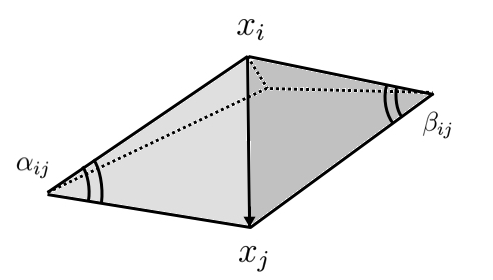
\includegraphics[width=0.3\textwidth]{figs/Chapter3/MyDesbrun.png}
		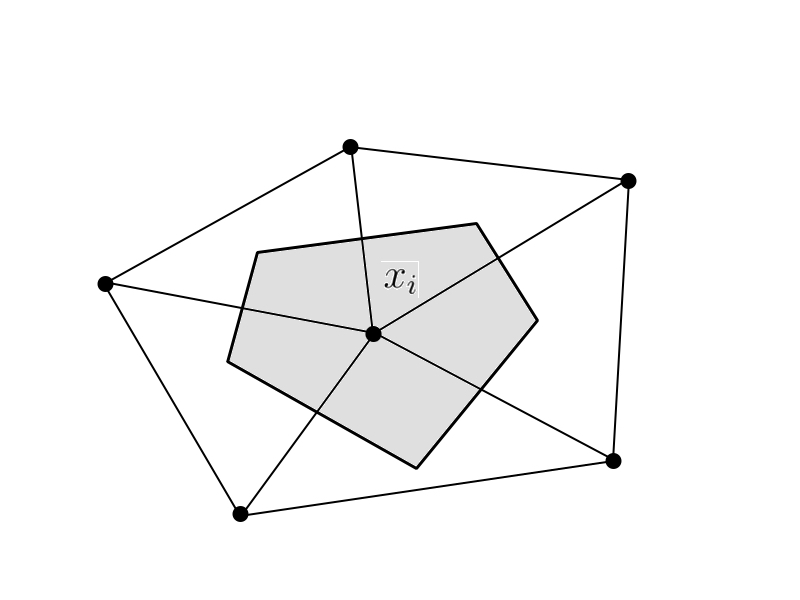
\includegraphics[width=0.3\textwidth]{figs/Chapter3/Voronoi}
	\end{center}
	\caption{One term of curvature normal formula and one Voronoi cell constructed around the vertex $x_i$}
\end{wrapfigure} 

where $A_i$ is the area of all the triangles of the mesh sharing the vertex $x_i$; $N_1(i)$ is the first ring of neighbors of the i-th vertex; $\alpha_{i j},\ \beta_{i j}$ are the angles of the triangles of the mesh that lie on the opposite side to the edge $(i,j)$ with respect to the vertex $x_i$ (Figure \ref{fig:Desbrun}). This is a geometric approach that relies on the intrinsic properties of the mesh constructed and is based on the continuous formulation of the curvature normal. Using equations \ref{eq:curvature normal} and \ref{eq:laplacian and curvature} it can be shown \cite{REUTER2009381} that this approach leads to a \textit{discrete Laplacian} with masses $d_i=A_i$ where $A_i$ is the area of all the triangles of the mesh with a vertex in $x_i$, and weights

$$w_{i j}=\frac{\cot \left(\alpha_{i j}\right)+\cot \left(\beta_{i j}\right)}{2}$$

Meyer et al. \cite{Meyer02discretedifferential-geometry} modify the masses of Desbrun et al. and set the masses $d_i$ to be equal to $a_{V}(i)$, where \(a_{V}(i)\) is the area of the polygon obtained by joining the circumcenters of the triangles surrounding vertex $i$ (i.e. the Voronoi cell).


\subsubsection{A graph alternative to the HKGL for the equiangular sampling}
Frossard et al. \cite{Frossard2017GraphBasedCO} to design a discrete Laplacian that is explicitly intended to work on the sphere with the equiangular sampling. They studied a way to build a graph to analyze image produce by omnidirectional cameras. In their work they assume that the image is sampled on the sphere on the equiangular sampling described in the above section. They start by considering the set $\mathcal G$ of all the possible graph where each node is connected just with 4 of its nearest neighbours (North, Sud, West, East) and propose a weighting scheme $w_{ij}$ specifically designed for the analysis of spherical signals such that the difference in the response to the polynomial spectral filter $\mathcal F = \mathbf L$ evaluated on images of the same object seen at different latitudes is minimized. In other words, they solve the minimization problem 

\begin{equation}\label{eq:minimization frossard}
	\min_{W\in\mathcal G} \left|\mathcal{F}\left(\mathbf{y}\left(v_{ e}\right)\right)-\mathcal{F}\left(\mathbf{y}\left(v_{ i}\right)\right)\right|
\end{equation}

for the adjacency matrix $W$, where $\mathbf y(v_i)$ is the image of the object on the sphere centered on the vertex $v_i$, and $\mathcal f\mathbf y(v_e)$ is the response of the filter at the vertex $v_e$ that lies at the same longitude of the vertex $v_i$ but on the equator. In their work they prove that the optimal weights solving the minimization problem \ref{eq:minimization frossard} are given by weights inversely proportional to the Euclidean distance between pixels
$$
w_{ij} = \frac{1}{\norm{v_i-v_j}}
$$

This construction is interesting since it is adapted to the equiangular sampling (where the Heat Kernel Graph Laplacian performed badly) and by construction of the set $\mathcal G$ it leads to a graph with only 4 neighbors per node, thus very sparse. In order to compare it to the Heat Kernel Graph Laplacian we show the same Power Spectrum analysis in figure \ref{fig:Frossard/Khasanova graph}. It can be appreciated how this construction performs way better than the Heat Kernel Graph Laplacian, having furthermore the big advantage of being naturally very sparse.
\begin{figure}[h!]
	\label{fig:Frossard/Khasanova graph}
	\centering
	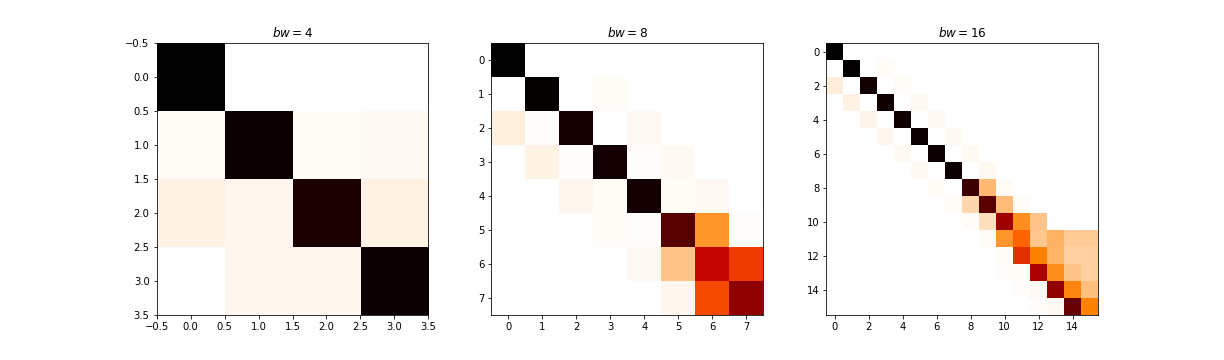
\includegraphics[width=0.9\textwidth]{../codes/02.HeatKernelGraphLaplacian/equiangular/equi_Khasanova_Frossard_full.png}
	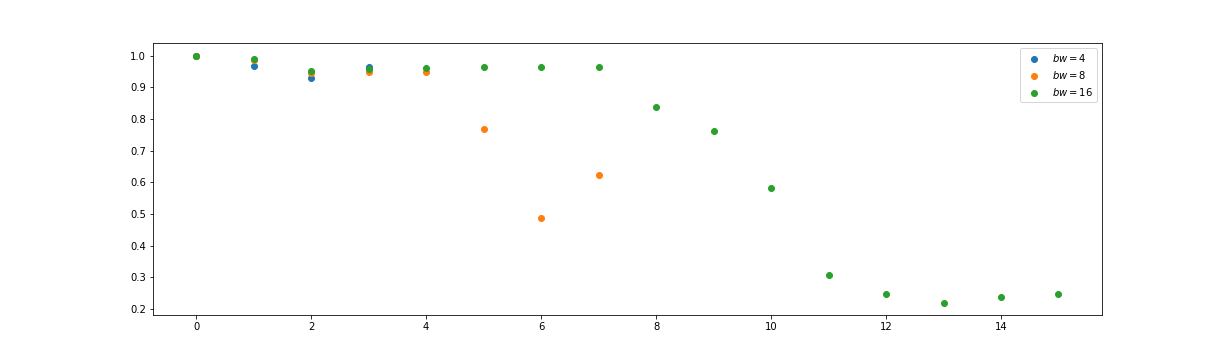
\includegraphics[width=0.9\textwidth]{../codes/02.HeatKernelGraphLaplacian/equiangular/equi_Khasanova_Frossard_full_diagonal.png}
	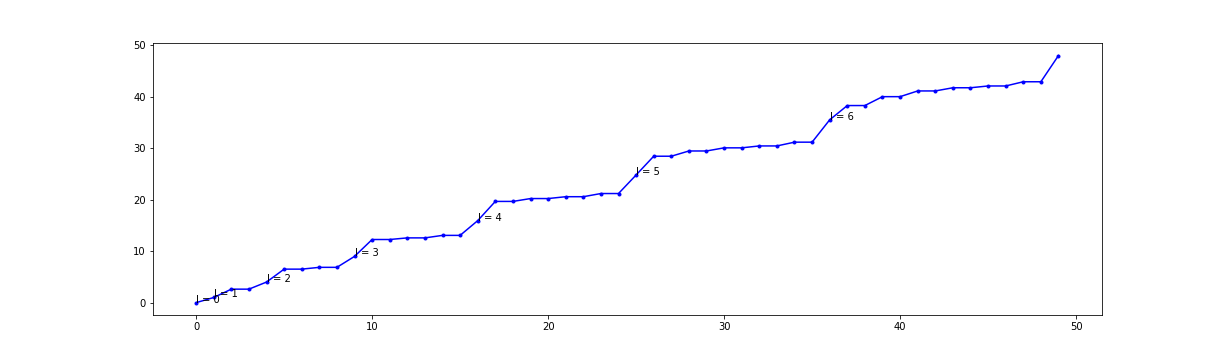
\includegraphics[width=0.9\textwidth]{../codes/02.HeatKernelGraphLaplacian/equiangular/equi_full_Khasanova_Frossard_eigenvalues_16.png}
	\caption{Frossard/Khasanova graph}
\end{figure}

\subsection{The Finite Element Method approximation of the Laplace-Beltrami operator on a manifold}\label{sec:Chapter3: Using the Finite Element Method to approximate the Laplace-Beltrami operator on a manifold}
The Finite Element Method is a numerical algorithm that implements the Galerkin method. In the Galerkin method we take the weak formulation of the eigenvalue problem, we reduce the spaces on which the problem is defined to spaces with a finite dimension, and through the linearity of the differential operator we transform the continuous problem into a finite dimensional, algebric eigenvalue problem that we can solve using the normal method of linear algebra. In this section we provide the necessary definitions and mathematical concepts necessary to properly introduce the weak formulation of the eigenvalue problem, the Galerkin method and finally the Finite Element Method. \\

A Banach space $(X, \norm{\cdot})$ is a normed vector space on the scalar field $F$ "big enough" such that for every Cauchy sequence $(x_n)\subset X$ there exist a $x\in X$ such that $x$ is the limit of $(x_n)$ in $X$ i.e. $\norm{x_n-x}\rightarrow 0$. A basis of $(X, \norm\cdot)$ is a minimal set of linearly independent vectors $\mathcal B \subset X$ such that every element of $X$ can be written as linear combination of the elements of $\mathcal B$. To perform Fourier analysis we are interested in those particular Banach spaces where we can define a notion of orthogonality between vectors. Such Banach spaces are called Hilbert spaces: $(X, \norm \cdot )$ is a Hilbert space when it is Banach and furthermore the norm $ \norm \cdot $ can be induced by a \textit{scalar product}: $\norm \cdot = \sqrt{\langle\cdot,\cdot\rangle}$. In this general context a scalar product is a function $\langle\cdot,\cdot\rangle: X\times X \rightarrow \mathbb F$ that is linear in the first argument, positive definite and conjugate symmetric. Through a scalar product we can define the notion of angle $\theta$ between two elements $x, y \in X$ through the following formula: 
$$
\cos \theta = \frac{\langle x, y\rangle}{\norm x \norm y}
$$ 
and in particular we can define the notion of orthogonality: two elements  $x, y \in X$ are orthogonal if and only if $\langle c, y\rangle=0$. We can now define what an \textit{orthonormal} basis of $X$ is: a basis $\mathcal B \subset X$ such that $\forall x, y \in \mathcal B, \norm x = \norm y = 1 \text{and } \langle x, y\rangle = 0$. Given an orthonormal basis $\mathcal B = \{b_i\}_{i\in I}$ we can write each vector in its \textit{Fourier series} 

\begin{equation}\label{eq:abstract fourier}
	x = \sum_{i\in I} \frac{\langle x, b_i\rangle}{\norm {x^2}}b_i
\end{equation}
If the set $I$ is countable the Hilbert space $(X, \norm\cdot)$ is called \textit{separable}. Having an orthonormal basis, and thus the possibility of representing each vector through its Fourier series \ref{eq:abstract fourier} enormously simplifies many problems.

\paragraph{Linear operators and bilinear forms} A \textit{linear operator} $L: X\to X$ on the Banach space $(X, \norm \cdot)$ is such that $L(\alpha x + \beta y) = \alpha L x + \beta L y$. $(x, \lambda)$ are called respectively \textit{eigenvector} and \textit{eigenvalue} of the linear operator $L$ is the image of $x$ is a rescaling of $x$ through a factor $\lambda$ i.e. $Lx = \lambda x$. The operator $L$ is called \textit{self-adjoint} if $\langle Lx, y\rangle = \langle x,Ly\rangle\ \  \forall x,y \in X$. Self-adjoint operators have two important properties: their eigenvalues are real, and two eigenvectors $x, y$ associated to different eigenvalues $\lambda, \mu$ are orthogonal. Indeed 
$\langle Lx, y\rangle = \langle x,Ly\rangle$
$\langle \lambda x, y\rangle = \langle x,\mu y\rangle$
$\lambda \langle  x, y\rangle = \mu \langle x, y\rangle$
that implies $ \langle  x, y\rangle = 0$
If the eigenvectors of a self-adjoint operator $L$ span the whole space $X$, than $L$ is called \textit{diagonalisable}.

A bilinear form on the vector space $X$ is a map $a(\cdot, \cdot): X\times X\to F$ that is linear with respect to both arguments. It is said to be \textit{strongly coercive} if $\exists\alpha>0:\ |a(x, x)|\geq \alpha \norm {x}^2$, and \textit{bounded} if $\exists M>0:\ |a(x, y)|\leq M \norm x \norm y$.
\subsubsection{Weak formulation of a PDE and Galerkin Method}
Galerkin's method is a method to approximate a continuous differential problem with a finite dimensional one. This method is proved to be well posed (i.e. there exist one and only one solution) that converges to the one of the continuous problem. To introduce this method it is useful to first state the famous Lax-Milgram theorem, a result of functional analysis that uses all but only the concepts that we have introduced so far:
\vspace{0.5cm}
\begin{theorem}[Lax-Milgram]
If \(a(\cdot, \cdot)\) is a bounded and strongly coercive bilinear form on the Hilbert space \(X\) then given \(u \in X\) there exist a unique solution $x$ to the following problem:
\begin{equation}\label{eq:variational abstract problem}
	\text{Find }x\in X\text{ such that } a(x, v)=\langle u, v\rangle \text{ for all } u \in X
\end{equation}
For such \(x\) one has \(\|x\| \leq \frac{1}{\alpha}\norm u\) where \(\alpha>0\) is the coercive constant \(a(v, v) \geq \alpha\norm v^{2} \forall v \in X ) .\)
\end{theorem} 
\vspace{0.5cm}
Our goal now is to explain how to write a differential problem like 
\begin{equation}\label{eq:strong form}
\text{Find }f\in C^2(\Omega) \text{ such that given }u\in C(\Omega)
\begin{cases}
-\partial_{x_1x_1}f(\mathbf x) - \partial_{x_2x_2}f(\mathbf x) = u(\mathbf x) & \mathbf x \in \Omega\\
f(\mathbf sx) =  0& \mathbf x \in \partial \Omega
\end{cases}
\end{equation}
in the form \ref{eq:variational abstract problem}. Let's multiply the differential equation times a sufficiently regular function $v$ that vanishes on $\partial \Omega$ and integrate on $\Omega$. Since the contribution of both $f$ and $v$ on the border $\partial \Omega$ is zero, integrating by parts we get

\begin{equation}\label{eq:int by parts}
	\int_\Omega \nabla f(\mathbf x)\cdot\nabla v(\mathbf x) d\mathbf x = \int_\Omega  u(\mathbf x)\cdot v(\mathbf x)d\mathbf x
\end{equation}

By defining $a(f, v):=	\int_\Omega \nabla f(\mathbf x)\cdot\nabla v(\mathbf x) d\mathbf x $ and taking the usual dot product \\$\langle u, v\rangle = \int_\Omega  u(\mathbf x)\cdot v(\mathbf x)d\mathbf x$ in the space of square-integrable functions $L^2(\Omega)$ equation \ref{eq:int by parts} can be written in the form of equation \ref{eq:variational abstract problem}. It remains to verify that $a(\cdot, \cdot)$ is actually bounded and coercive, and to choose a space $X$ that is carefully constructed to be "big enough" to include those functions such that $\nabla f \in L^2(\Omega)$ and to be Hilbert with respect to the $L^2$ product $\langle\cdot,\cdot\rangle$, and at the same time "small enough" to include only those functions that are equal to 0 on the boundary of $\Omega$. It turn out that such Hilbert space exists, it is called $H^1_0(\Omega)$ and it is such that, once restricted to the continuous functions $C(\Omega)$, it contains only those functions that vanish on $\delta \Omega$ i.e. $f\in H^1_0(\Omega)\cap C(\Omega) \implies \left.f(\mathbf x)\right|_{\partial\Omega}=0$. This means that thanks to Lax-Milgram's theorem the problem

\begin{equation}\label{eq:final variational form}
	\text{Given }u\in L^2(\Omega)\text{ find }f\in H^1_0(\Omega)\text{such that }\int_\Omega \nabla f(\mathbf x)\cdot\nabla v(\mathbf x) d\mathbf x = \int_\Omega  u(\mathbf x)\cdot v(\mathbf x)d\mathbf x\quad \forall v\in H^1_0(\Omega)
\end{equation}

has one and only one solution. To have this result (existence and uniqueness of the solution) we had to pay the price of looking for such result in a much bigger space than $C^2(\Omega)$. This means that a priori our solution $f$ to problem \ref{eq:final variational form} could not be a solution to problem \ref{eq:strong form}! However, there are regularity results that we omit that assure that if the forcing term $u$ is regular enough, than also the solution $f$ will be regular and thus the strong form problem and the weak form problem are actually equivalent, and thus solving \ref{eq:final variational form} eventually leads to solving \ref{eq:strong form}.

However, now that we know that a solution exists, we need to compute it! Computing it analytically is often impossible; Galerkin's method in a mathematical tool provide us a way to compute an approximation of the solution $f$.

Take the variational problem \ref{eq:variational abstract problem}, but restrict the ambient space to be a finite dimensional subspace of $X$, say $V_h = \text{span}\{phi_0, ..., phi_{n-1}\}$.

\subsubsection{The eigenvalue problem on a manifold}
[Weak formulation of the eigenvalue problem on the sphere, generalized eigenvalue problem, lumping of the mass matrix, discussion on the solvers]

The eigenvalue problem \ref{eq:continous eigenvalue problem} can be also formulated for a closed manifold in the following \textit{weak form}

\begin{equation}\label{eq:weak eigenvalue problem}
sdfq
\end{equation}

Lumping of the mass matrix
\begin{figure}[h]
	\label{fig:Lumping}
	\centering
	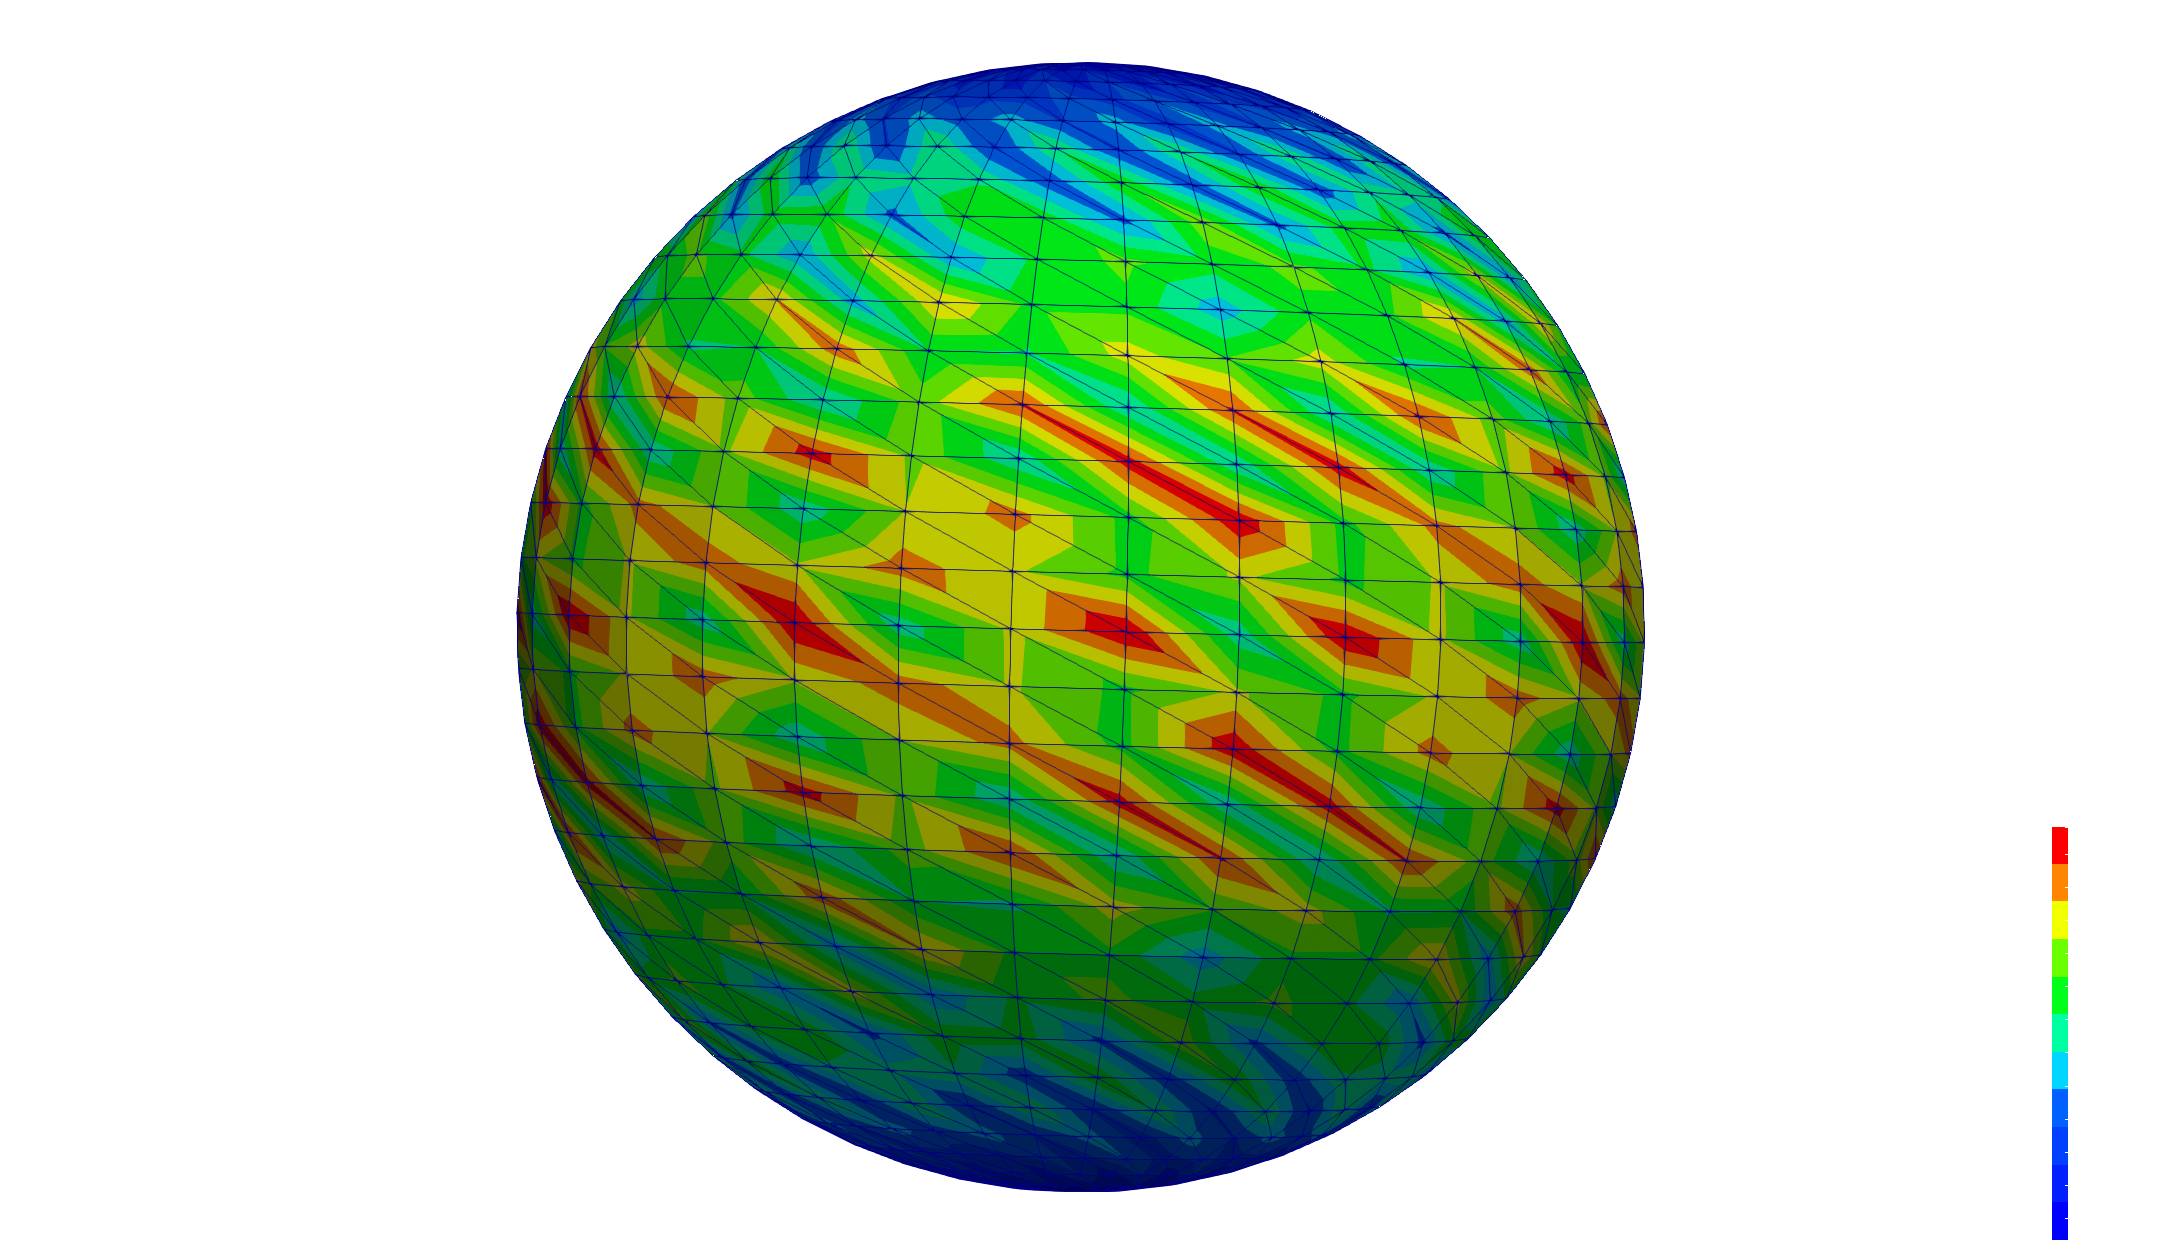
\includegraphics[width=0.9\textwidth]{figs/Chapter3/B_diagonal.png}
	\caption{Diagonal of the lumped mass matrix}
\end{figure}


\subsubsection{Manifold Harmonic Transform}



\subsection{Results}
\label{sec:Chapter3: Results}
We implemented with FEniCS the eigenvalue problem \ref{eq:FEM eigenvalue problem}
\subsubsection{Alignment of eigenspaces and analysis of the spectra}

\paragraph{HEALPix}
\begin{figure}[h]
	\label{fig:HeatKernelGraphLaplacianHealpix}
	\centering
	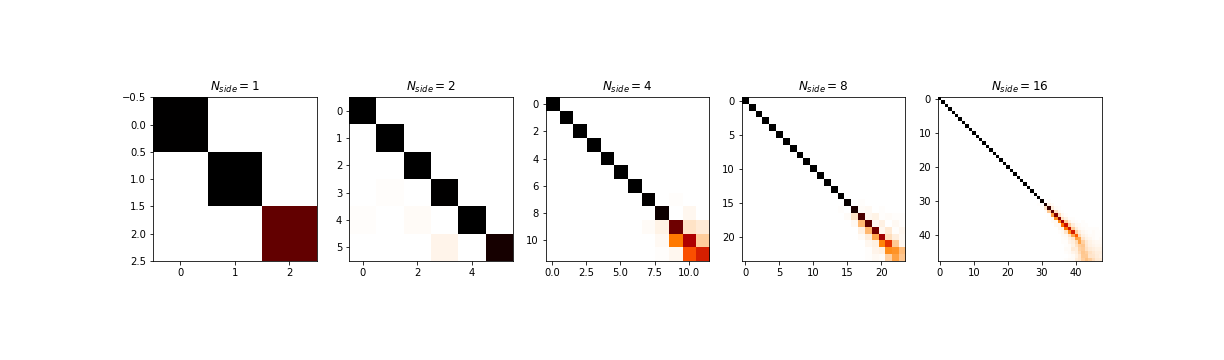
\includegraphics[width=0.4\textwidth]{../codes/02.HeatKernelGraphLaplacian/HEALPix/06_figures/optimal_thresholded.png}
	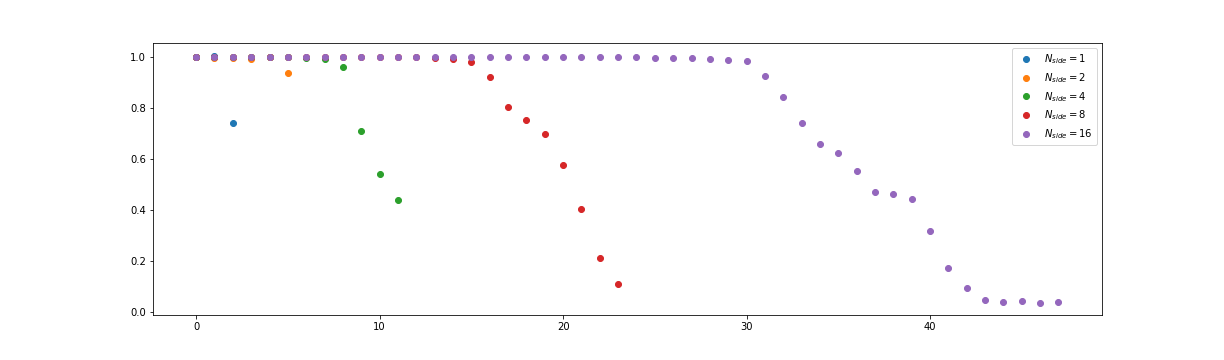
\includegraphics[width=0.4\textwidth]{../codes/02.HeatKernelGraphLaplacian/HEALPix/06_figures/optimal_thresholded_diagonal.png}	
	\caption{Heat Kernel Graph Laplacian on HEALPix}
\end{figure}

\begin{figure}[h]
	\label{fig:FEMHealpix}
	\caption{Linear FEM Laplacian on HEALPix}
	\centering
	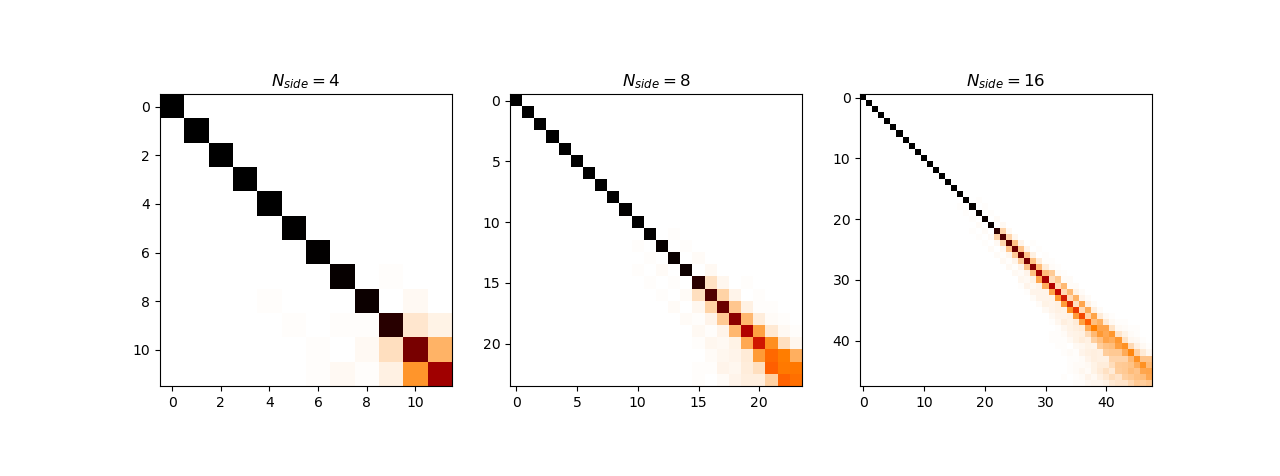
\includegraphics[width=0.4\textwidth]{../codes/03.FEM_laplacian/HEALPix/img/linearFEM.png}
	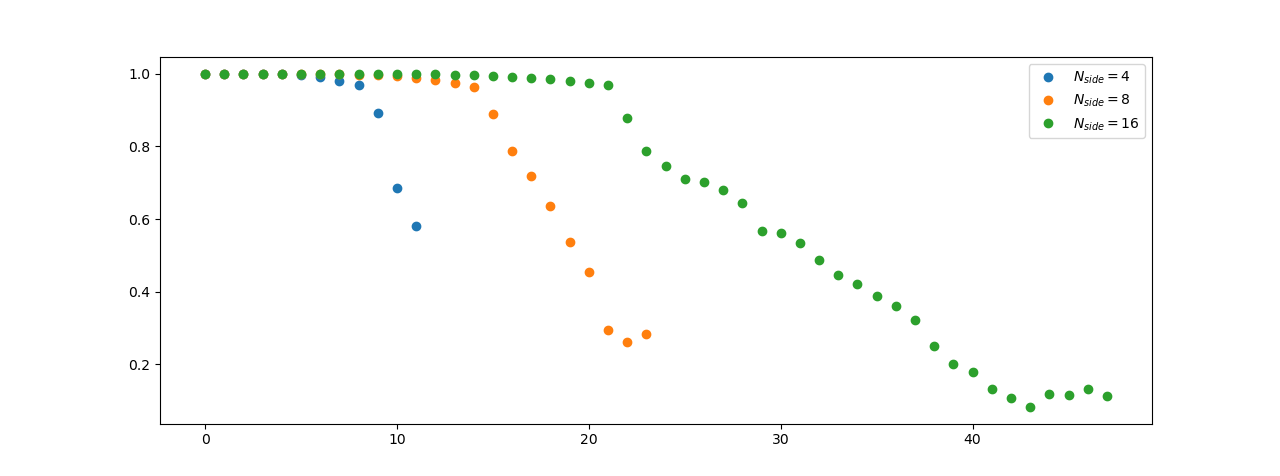
\includegraphics[width=0.4\textwidth]{../codes/03.FEM_laplacian/HEALPix/img/linearFEM_diagonal.png}	
	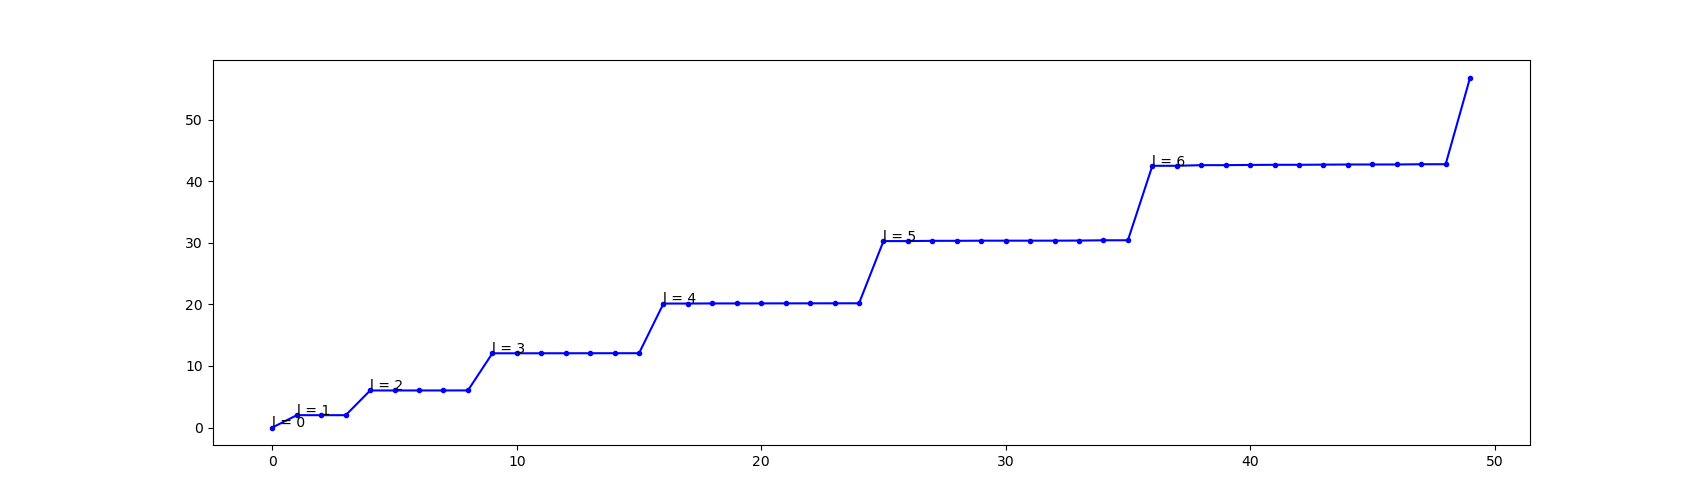
\includegraphics[width=0.4\textwidth]{../codes/03.FEM_laplacian/HEALPix/img/FEM_eigenvalues_16.png}	 
\end{figure}

\paragraph{Equiangular}
\begin{figure}[h]
	\label{fig:HeatKernelGraphLaplacianEquiangular}
	\caption{Heat Kernel Graph Laplacian on equiangular sampling}
	\centering
	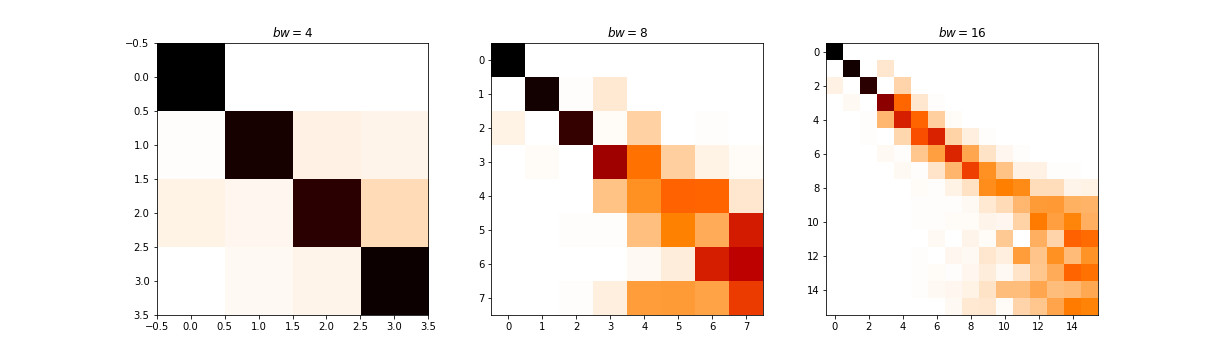
\includegraphics[width=0.4\textwidth]{../codes/02.HeatKernelGraphLaplacian/equiangular/equi_full.png}
	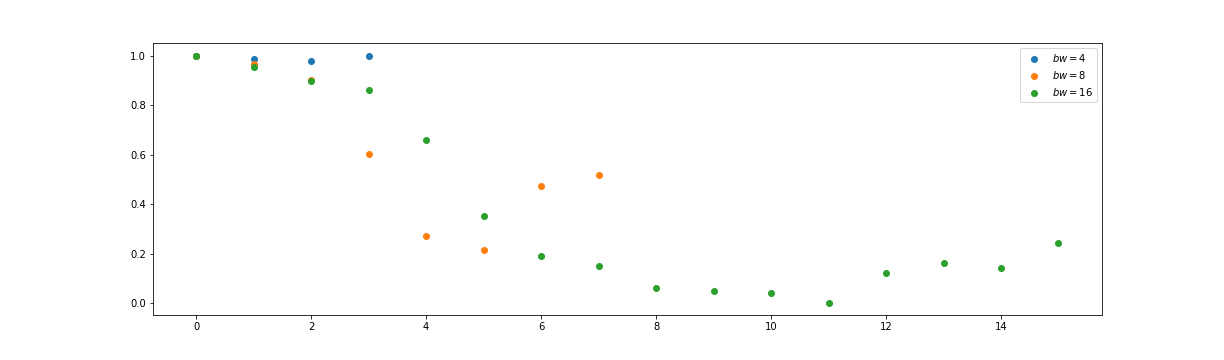
\includegraphics[width=0.4\textwidth]{../codes/02.HeatKernelGraphLaplacian/equiangular/equi_full_diagonal.png}	
	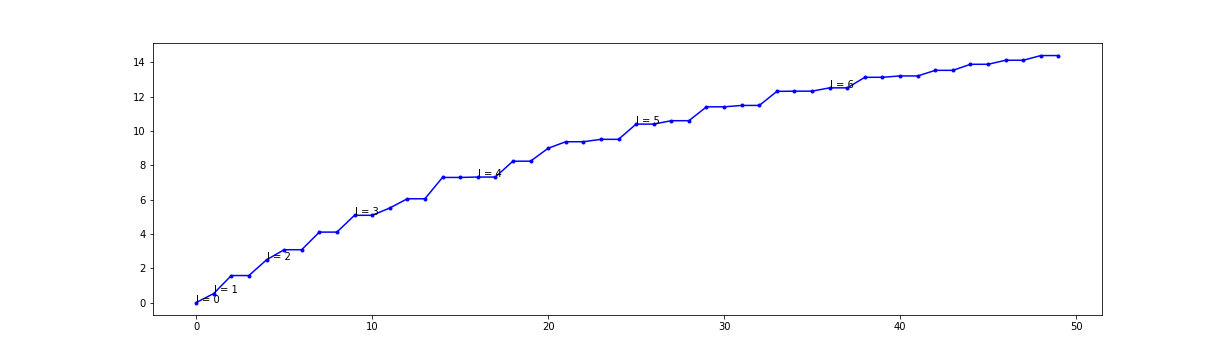
\includegraphics[width=0.4\textwidth]{../codes/02.HeatKernelGraphLaplacian/equiangular/equi_full_eigenvalues_16.png}	
\end{figure}


\begin{figure}[h]
	\label{fig:FEMequiangular}
	\caption{Linear FEM Laplacian on equiangular sampling}
	\centering
	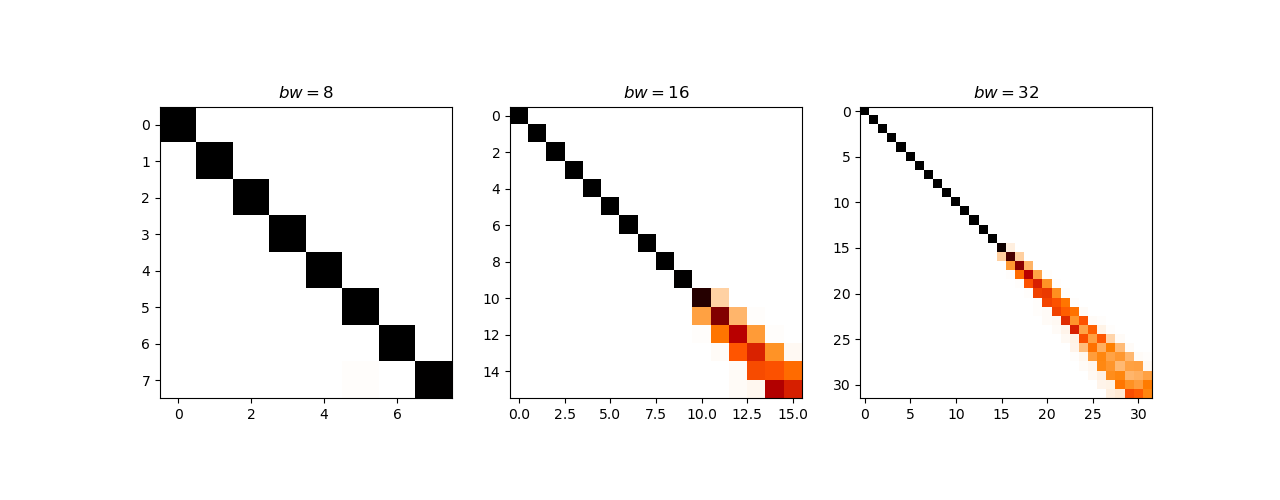
\includegraphics[width=0.4\textwidth]{../codes/03.FEM_laplacian/equiangular/normal/img/linearFEM.png}
	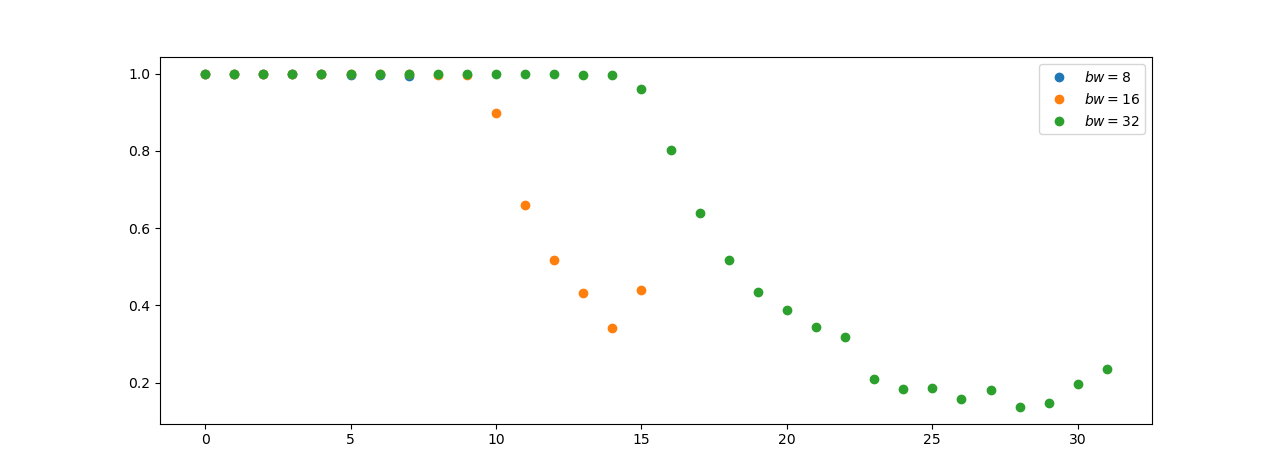
\includegraphics[width=0.4\textwidth]{../codes/03.FEM_laplacian/equiangular/normal/img/linearFEM_diagonal.png}	
	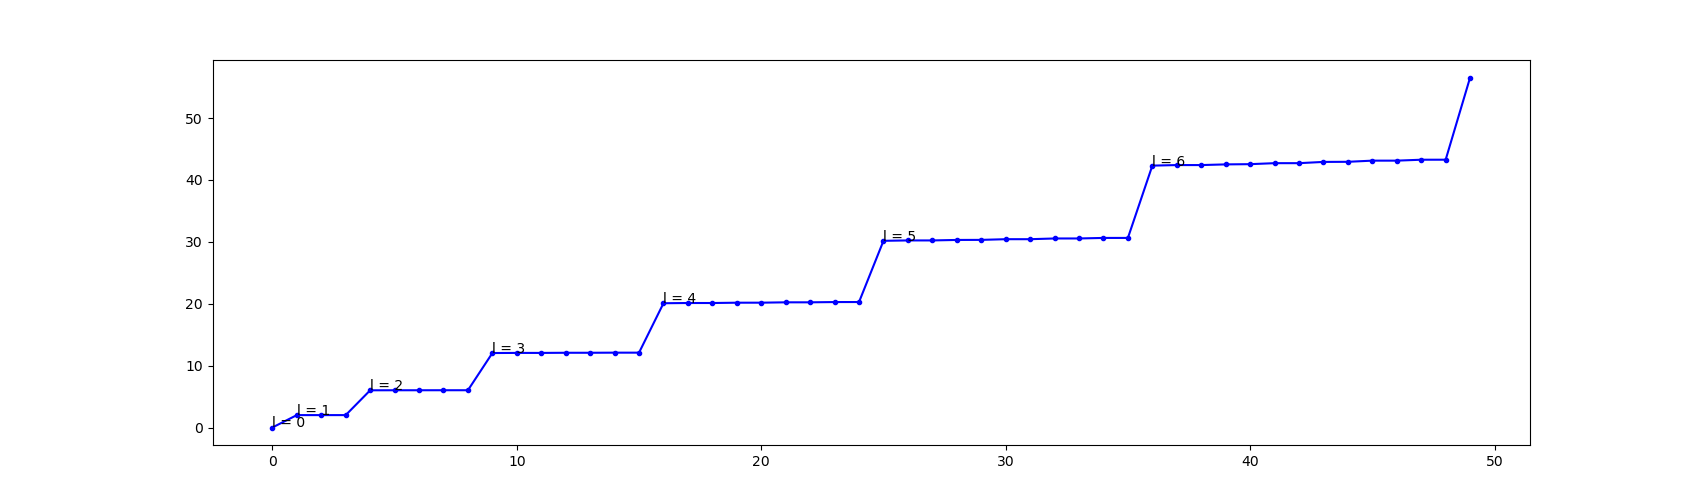
\includegraphics[width=0.4\textwidth]{../codes/03.FEM_laplacian/equiangular/normal/img/FEM_eigenvalues_16.png}	
\end{figure}

\paragraph{Lumping the mass matrix}


\begin{figure}[h]
	\label{fig:FEMequiangularLumped}
	\caption{Lumped Linear FEM Laplacian on equiangular sampling}
	\centering
	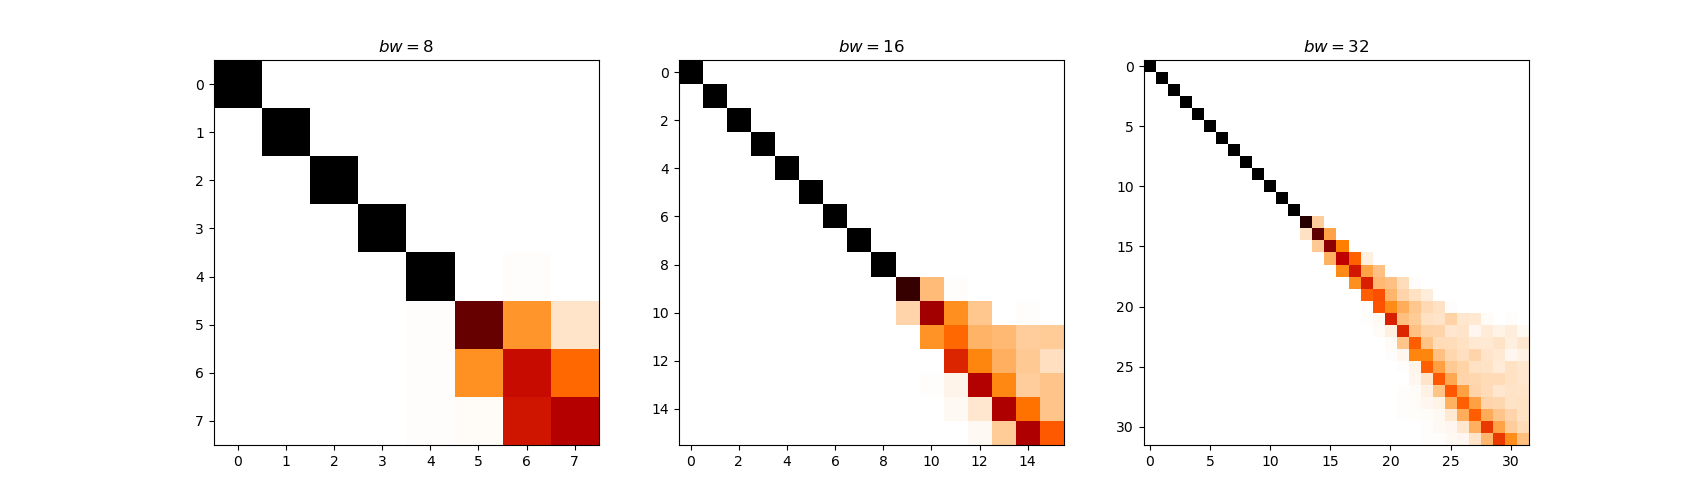
\includegraphics[width=0.4\textwidth]{../codes/03.FEM_laplacian/equiangular/mass_lumping/BL/img/linearFEM.png}
	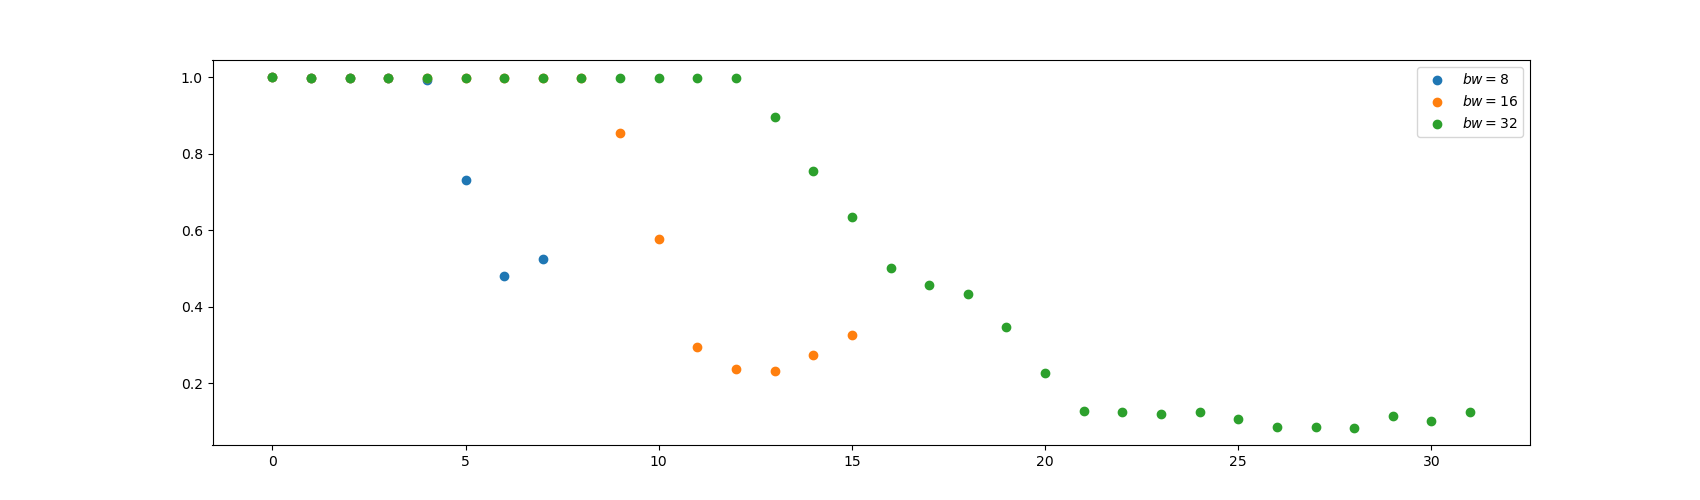
\includegraphics[width=0.4\textwidth]{../codes/03.FEM_laplacian/equiangular/mass_lumping/BL/img/linearFEM_diagonal.png}	
	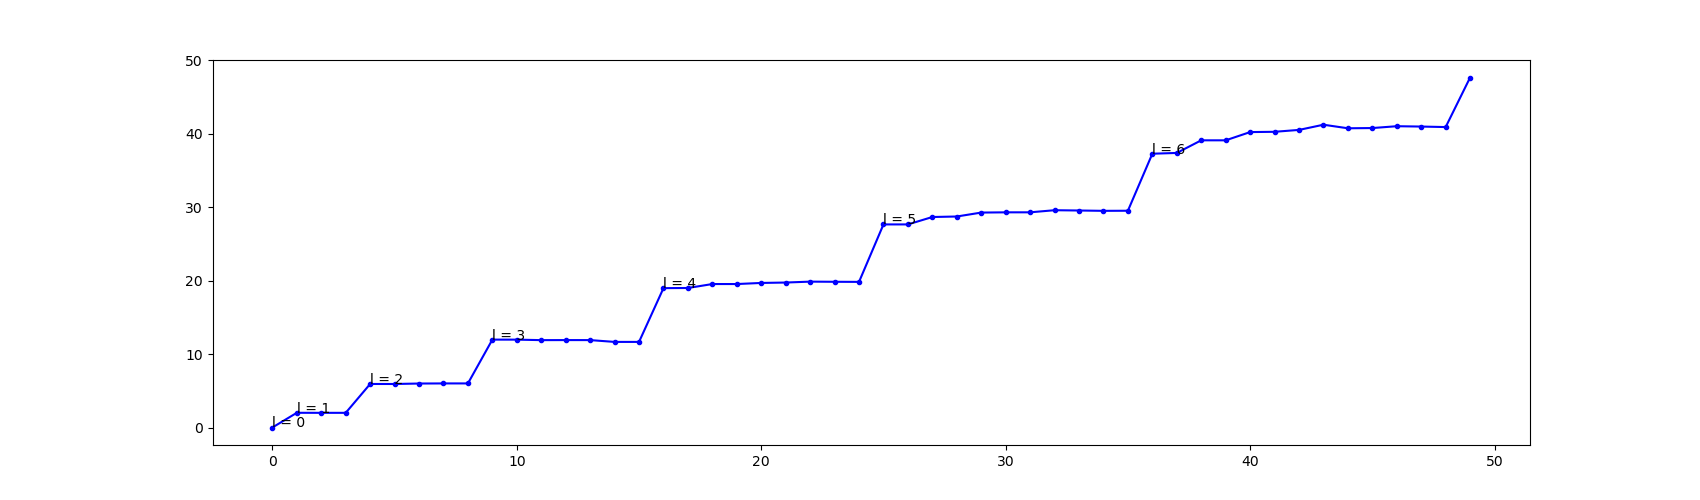
\includegraphics[width=0.4\textwidth]{../codes/03.FEM_laplacian/equiangular/mass_lumping/BL/img/FEM_eigenvalues_32.png}	
\end{figure}

\begin{figure}[h]
	\label{fig:symmetricFEMequiangularLumped}
	\caption{Symmetric Lumped Linear FEM Laplacian on equiangular sampling}
	\centering
	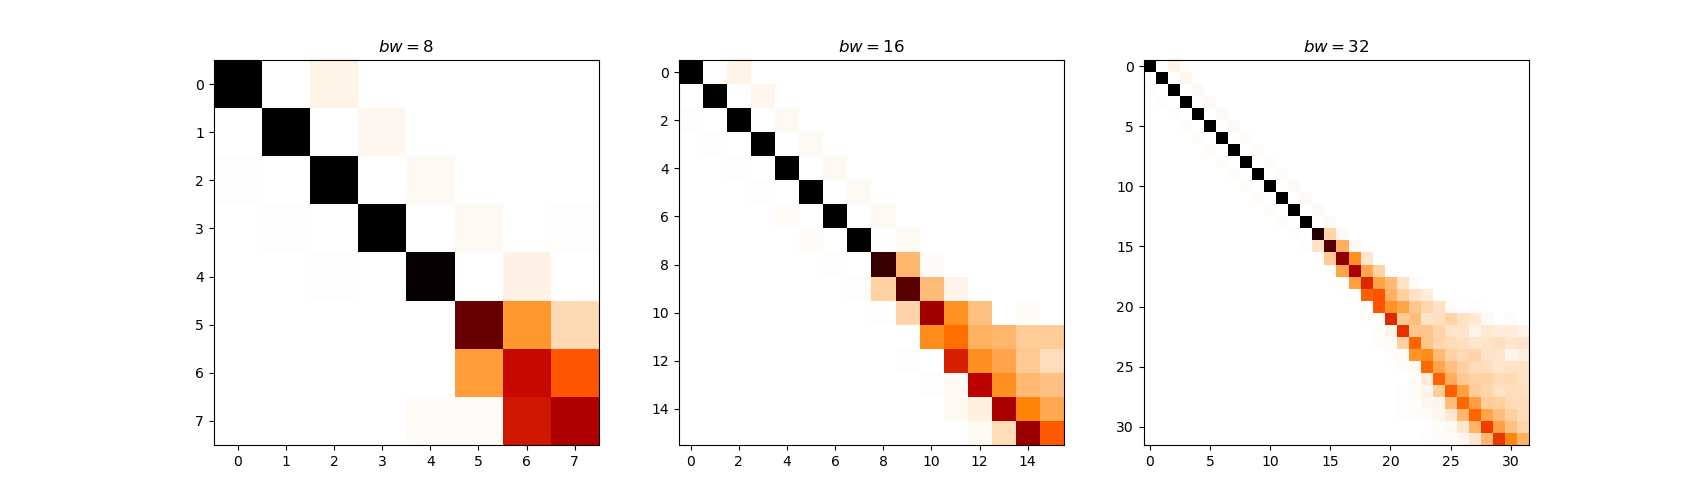
\includegraphics[width=0.4\textwidth]{../codes/03.FEM_laplacian/equiangular/mass_lumping/BLB/img/linearFEM.png}
	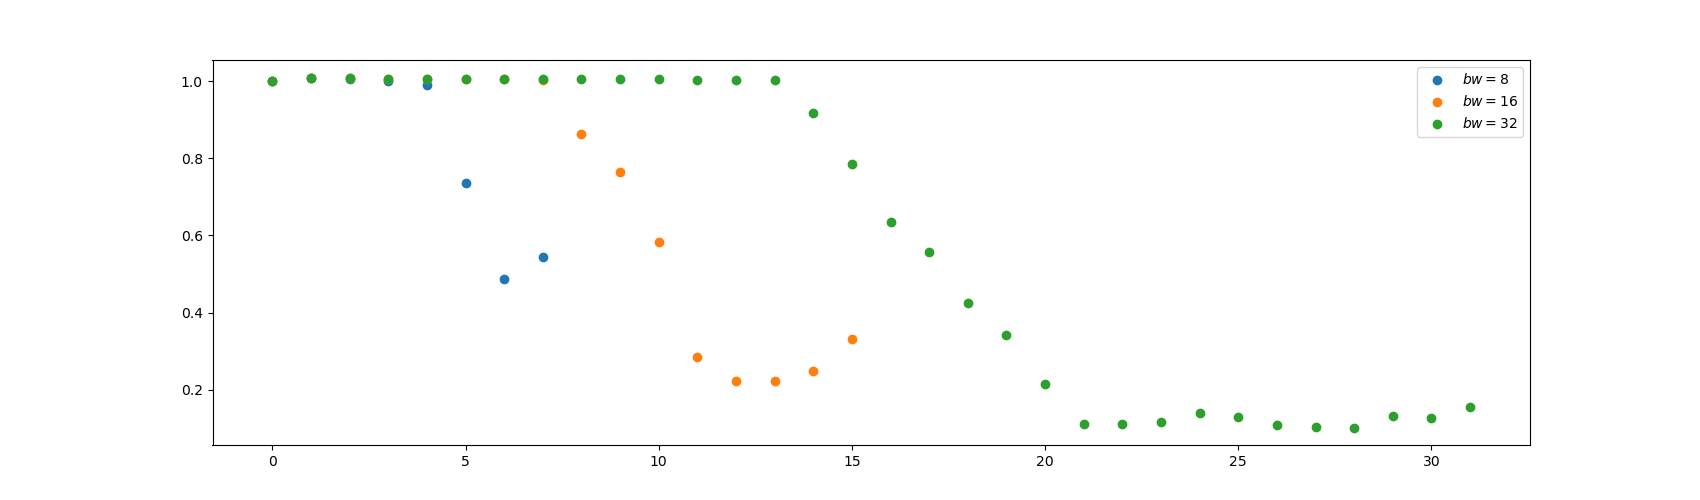
\includegraphics[width=0.4\textwidth]{../codes/03.FEM_laplacian/equiangular/mass_lumping/BLB/img/linearFEM_diagonal.png}	
	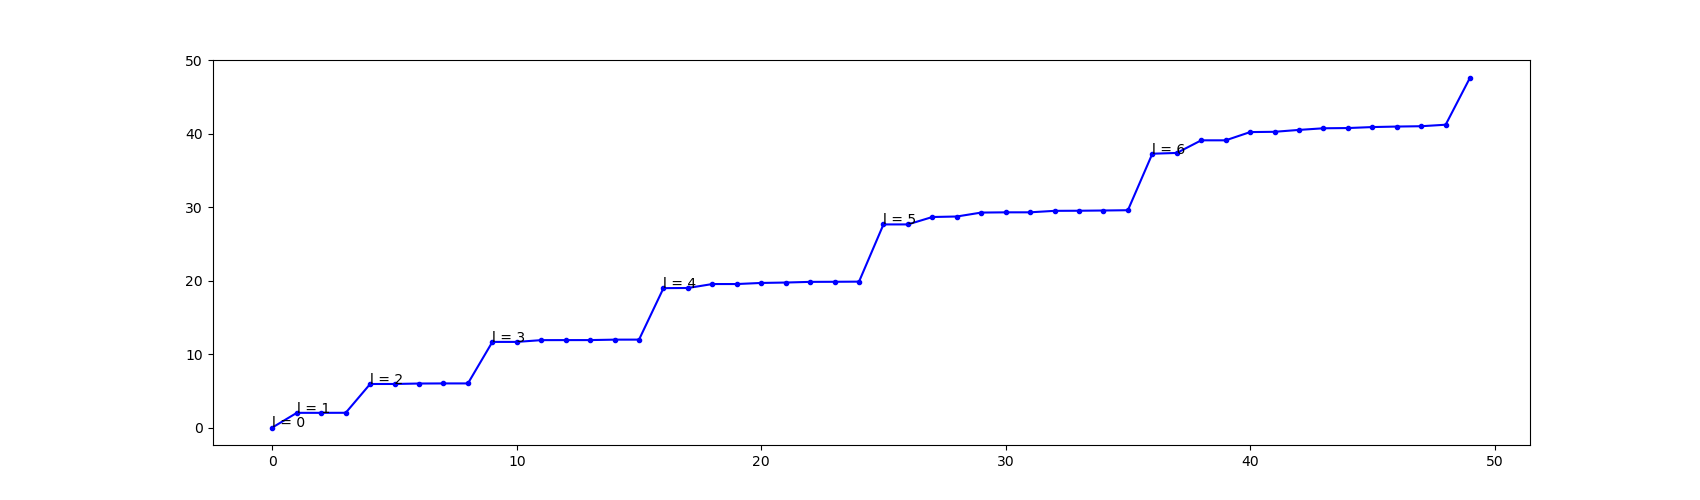
\includegraphics[width=0.4\textwidth]{../codes/03.FEM_laplacian/equiangular/mass_lumping/BLB/img/FEM_eigenvalues_32.png}	
\end{figure}
\subsubsection{Diffusion with the exponential matrix}


\begin{figure}[h]
	\label{fig:FEM lumped symmetric diffusion on equiangular sampling}
	\centering
	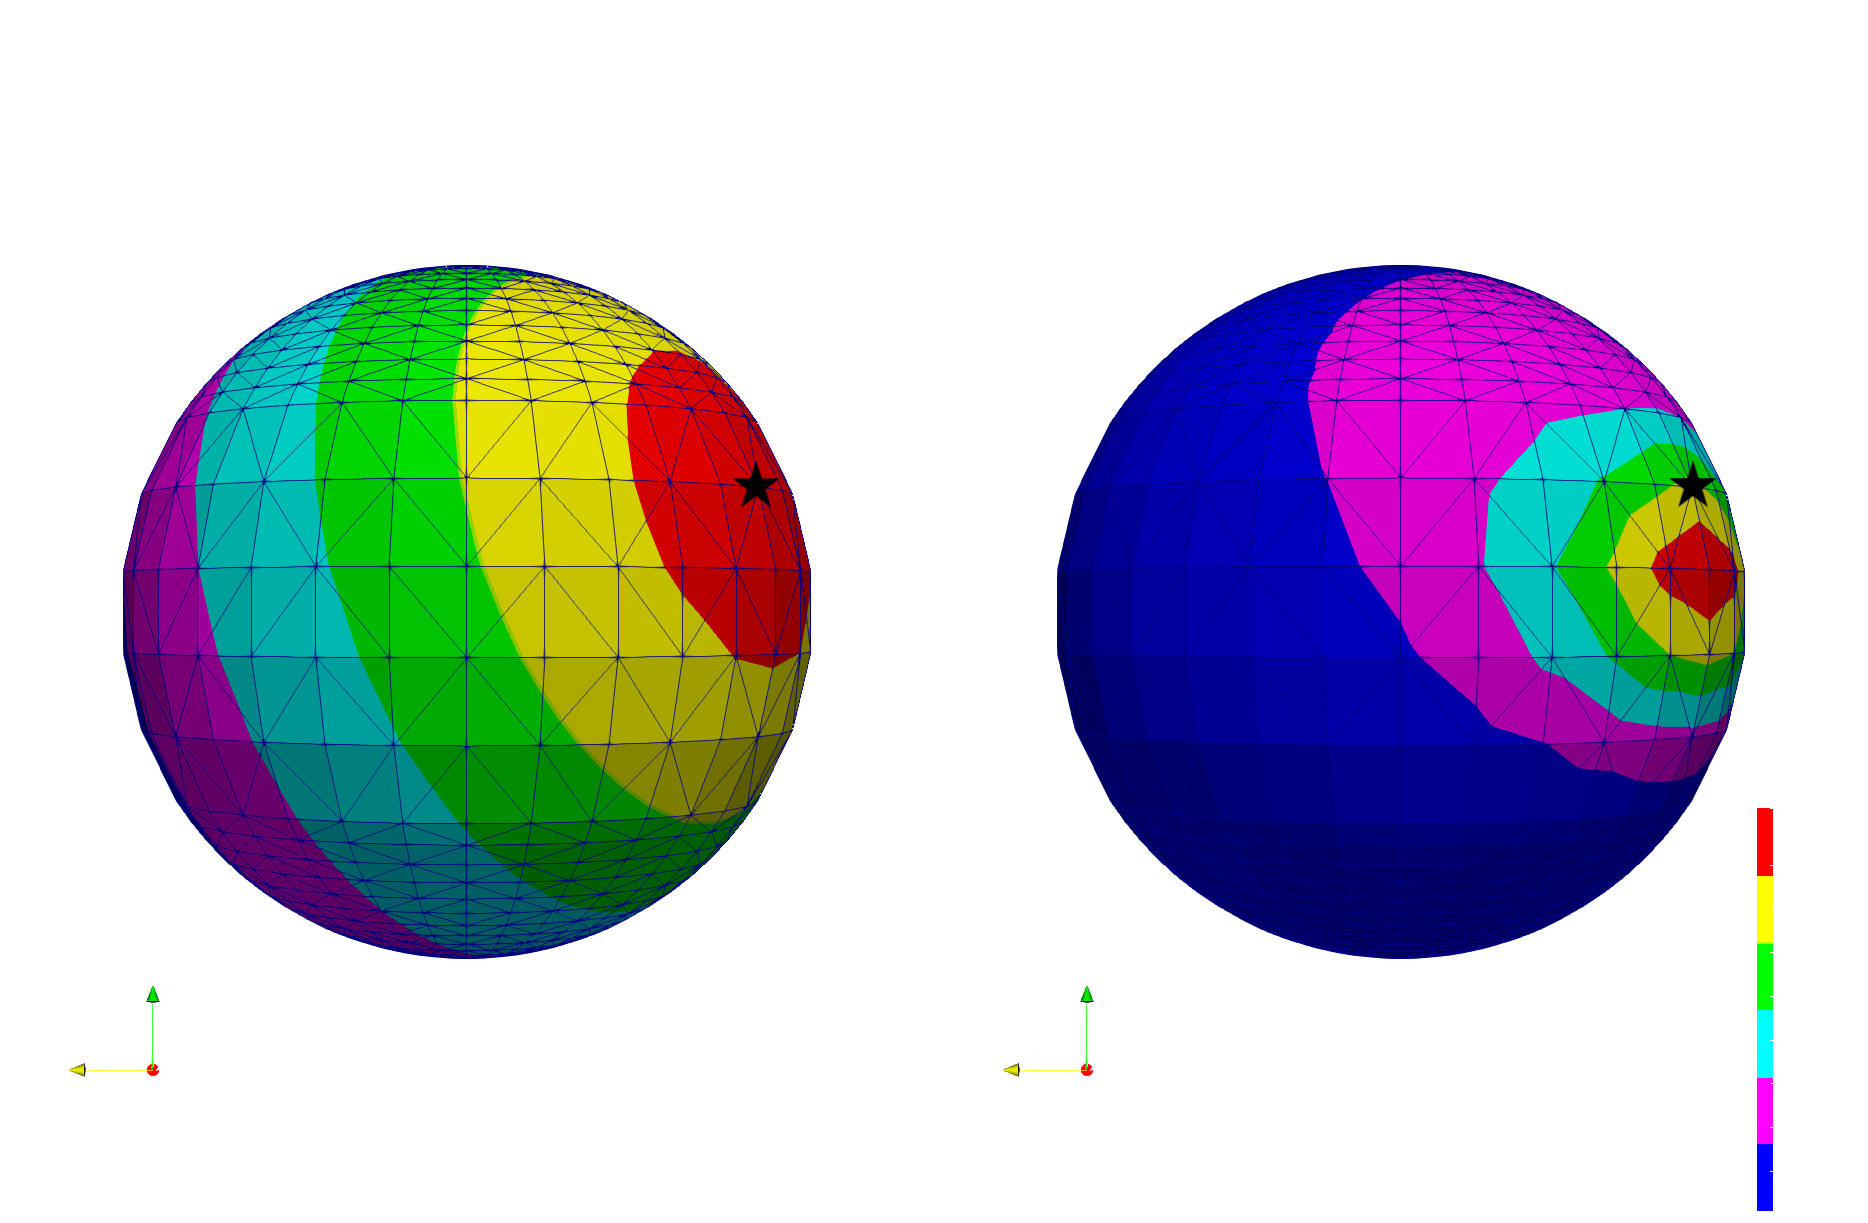
\includegraphics[width=0.9\textwidth]{figs/Chapter3/diffusion.png}
	\caption{FEM and graph diffusion on an irregular sampling}
\end{figure}

\subsubsection{Equivariance error}





